\section{Analysis and Methodology}
\label{sec:analysis_method}

In this section, we present the structural analysis and algorithmic design of our approach. As conceptually illustrated in \textbf{Figure~\ref{fig:theory_gap}}, \textcolor{blue}{we analyze a winner-action Gaussian distillation objective that exhibits a variance-expanding gradient tendency under the stated local assumptions, and contrast its continuous projection with the bounded discretization error of a support-aligned categorical policy} (\S\ref{sec:gauss_failure}). To resolve this mismatch, we introduce Iterative Gumbel Planning (IGP), which natively aligns the policy support with the discrete search candidates (\S\ref{sec:igp}), trading the continuous projection error for a rigorously bounded discretization error (\S\ref{sec:tradeoff}).

\subsection{Why Gaussian policies fail under search-based distillation}
\label{sec:gauss_failure}

Consider a Gaussian policy with diagonal covariance $\beta_\theta(\cdot\mid s)=\mathcal{N}(\mu,\mathrm{diag}(\sigma^2))$ at a fixed state $s$. Action samples are drawn via reparameterization,
$
    a_k=\mu+\sigma\odot\epsilon_k,\quad \epsilon_k\overset{i.i.d.}{\sim}\mathcal{N}(0, I),\quad k=1,\ldots,K,
$
and the winner action is the candidate maximizing the search-estimated value $\hat Q$:
$
    a_{\mathrm{sel}}\in\mathop{\arg\max}_{k\in\{1,\ldots,K\}}\hat Q(s,a_k).
$
Following the winner-based maximum-likelihood loss in Gumbel MuZero~\citep{danihelka2022policy}, the policy update maximizes the log-likelihood at the winner:
\begin{equation}
    \mathcal{L}(\mu,\sigma;s)=-\log\beta_\theta(a_{\mathrm{sel}}\mid s).
    \label{eq:winner_mle_loss}
\end{equation}
Distilling a single winner into the Gaussian via~\eqref{eq:winner_mle_loss} is itself a projection step: a finite-support search target is fit by a continuous density. \textcolor{blue}{The following result characterizes the expected directional pressure on the scale parameter under a local first-order model.}

\begin{wrapfigure}{r}{0.6\textwidth}
    \centering
    \vspace{-10pt}
    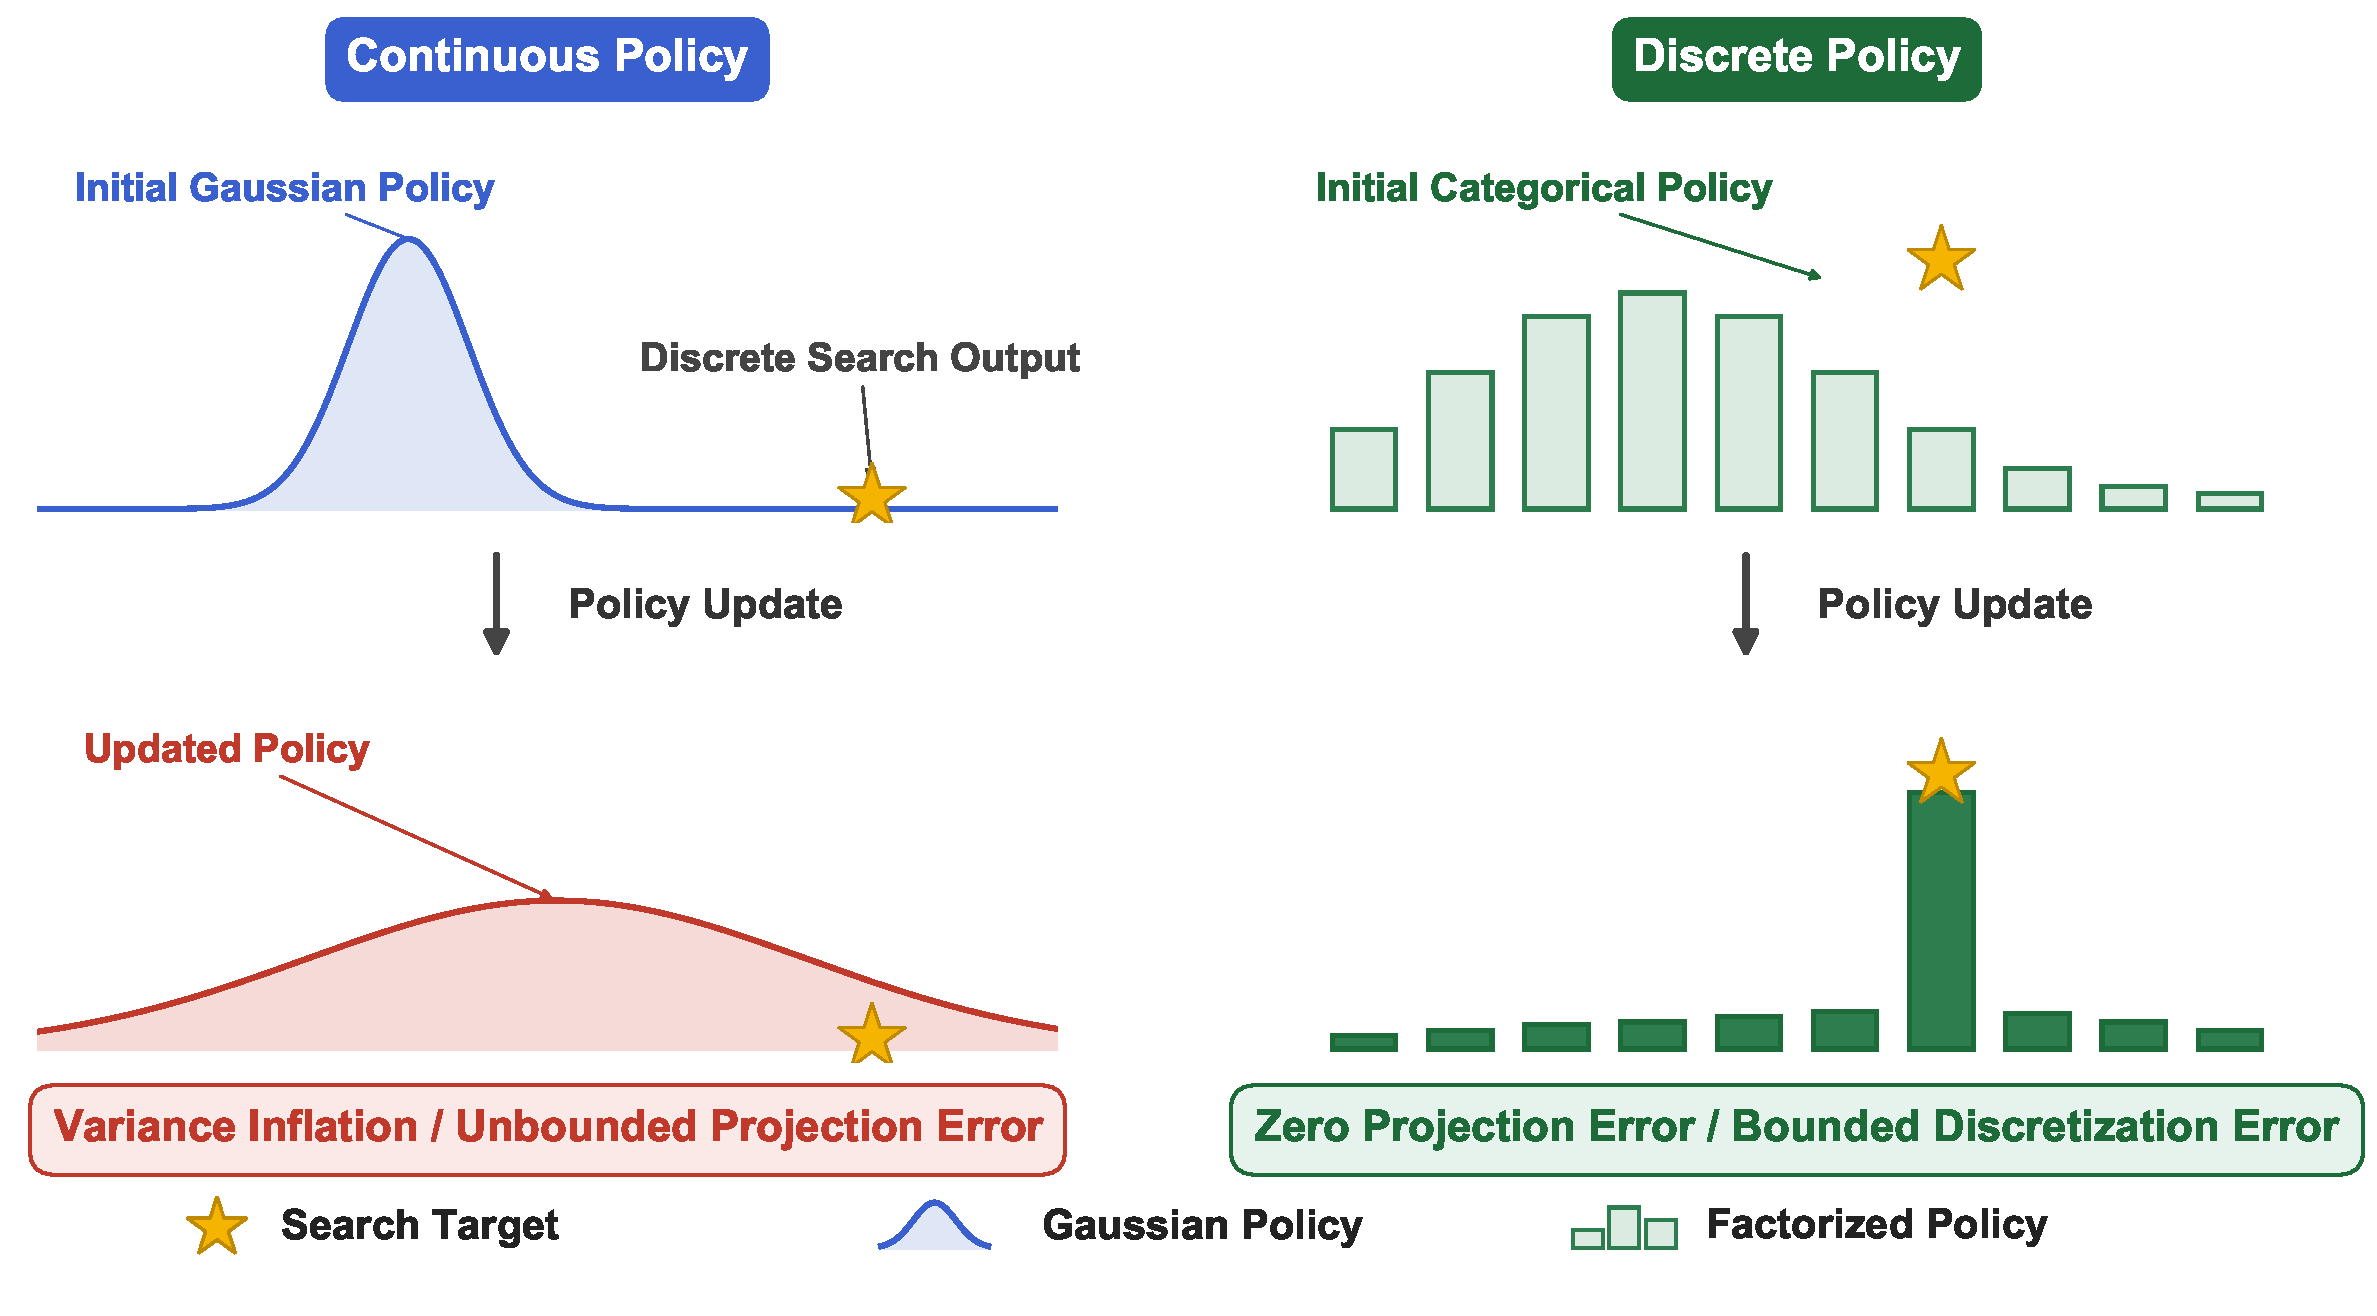
\includegraphics[width=0.6\textwidth]{figs/error.pdf}
    \caption{\textbf{Error trade-off in search-guided policy improvement.} (\textit{Left}) Gaussian distillation inherently inflates policy variance due to an unbounded projection error. (\textit{Right}) Our factorized discrete policy naturally aligns with the search support for exact distillation, replacing this unbounded error with a bounded discretization error.}
    \label{fig:theory_gap}
    \vspace{-10pt}
\end{wrapfigure}

\begin{proposition}[Directional inflation of Gaussian policy variance]
\label{prop:gaussian_var_inflation}
Assume the action value admits a local first-order approximation around $\mu$,
\[
\hat Q(s,a)\approx \hat Q(s,\mu)+g^\top(a-\mu)+o(\|a-\mu\|),\quad g\neq 0.
\]
Let $w=\sigma\odot g$, and let the winner $a_{\mathrm{sel}}$ be treated as a fixed target in the policy update. Then under~\eqref{eq:winner_mle_loss},
\[
\mathbb{E}\!\left[\frac{\partial \mathcal L}{\partial \log\sigma_i}\right]
=
-\frac{w_i^2}{\|w\|^2}\!\left(\mathbb{E}[\epsilon_{(K)}^2]-1\right)
\le 0,
\]
where $\epsilon_{(K)}=\max_{1\le k\le K}\epsilon_k$ with $\epsilon_k\overset{i.i.d.}{\sim}\mathcal{N}(0,1)$. The inequality is strict whenever $w_i\neq 0$ and $K\ge 3$.
\end{proposition}

{\color{blue}\begin{remark}[Weighted search targets]
The same scale tendency is not restricted to a one-hot winner target. For fixed normalized search weights $q_k$ and
\[
\mathcal L_q=-\sum_{k=1}^{K}q_k\log\mathcal N
\!\left(a_k;\mu,\operatorname{diag}(\sigma^2)\right),
\qquad \sum_k q_k=1,
\]
the per-dimension scale gradient is
\[
\frac{\partial\mathcal L_q}{\partial\log\sigma_i}
=1-\sum_{k=1}^{K}q_k\epsilon_{k,i}^{2}.
\]
Thus the update expands variance whenever search places sufficient mass on candidates with above-baseline standardized displacement; winner-action MLE is the one-hot special case. A quadratic variance penalty adds $2\lambda\sigma_i^2$ to this gradient, creating a task- and stage-dependent trade-off between suppressing inflation and preserving proposal diversity.
\end{remark}}

The winner is sampled from $\beta_\theta$ and almost surely does not coincide with $\mu$, so the maximum-likelihood objective raises $\beta_\theta(a_{\mathrm{sel}}\mid s)$ via two mechanisms: shifting $\mu$ toward $a_{\mathrm{sel}}$, and enlarging $\sigma$ to raise the density at $a_{\mathrm{sel}}$. \textcolor{blue}{Proposition~\ref{prop:gaussian_var_inflation} identifies this update-level variance-expanding mechanism, while Figure~\ref{fig:var_comp}(a) shows that it accumulates into a sustained training-time effect under practical finite-budget learning.} The full multi-dimensional proof is in Appendix~\ref{app:proof_of_var_inflation_multi_dim}.

We next show that variance inflation translates into a return gap, even at a converged policy mean.

\begin{proposition}[Inflated variance lowers $Q$]
\label{prop:inf_var_lower_Q}
Suppose the proposal policy is converged in the sense that $\mu=a^*$, and $Q(s,a)$ is locally $m$-strongly concave around $a^*$, a standard regularity assumption near a local optimum. Then
\[
\mathbb{E}_{a\sim\beta_\theta(\cdot\mid s)}[Q(s,a)]
\le
Q(s,a^*) - \frac{m}{2}\sum_i \sigma_i^2.
\]
\end{proposition}

\begin{corollary}[Return degradation under persistent variance inflation]
\label{cor:persistent_variance_return_gap}
If the local concavity condition in Proposition~\ref{prop:inf_var_lower_Q} holds along states in the visitation distribution $d^\pi$, then
\[
J(\pi^*)-J(\pi)
\ge
\frac{m}{2(1-\gamma)}\,\mathbb{E}_{s\sim d^\pi}\!\left[\sum_{i} \sigma_i^2\right].
\]
\end{corollary}

\textcolor{blue}{Under the local concavity assumptions, sustained policy variance induces a return gap proportional to $\sum_i\sigma_i^2$. Figure~\ref{fig:var_comp}(a) empirically demonstrates that the elevated variance persists over the practical training horizon, making this bound operational for the evaluated setting.} Proofs are in Appendix~\ref{app:proof_inf_var_lower_Q_ret}. This motivates aligning the policy support with the search candidates, which we develop next.


\subsection{Iterative Gumbel Planning}
\label{sec:igp}

To avoid the variance inflation analyzed in \S\ref{sec:gauss_failure}, we represent the policy on the same finite support that the search operates on. We instantiate this idea as \textbf{Iterative Gumbel Planning (IGP)}, with four components: a per-dimension factorized categorical policy, Gumbel Top-$K$ candidate sampling, search-output distillation, and multi-round root refinement.

\textbf{Per-dimension factorized categorical policy.}
For a continuous-control task with $|A|$ action dimensions and bounded action space $[-1,1]^{|A|}$, we discretize each dimension into $V$ bins with centers $\{c_v\}_{v=1}^{V}\subset[-1,1]$, giving a grid resolution $\Delta=2/V$. The policy network outputs per-dimension logits $p_\theta(s)\in\mathbb{R}^{|A|\times V}$, where $p_{\theta,j,v}(s)$ is the logit of bin $v$ on dimension $j$. The policy is the product of $|A|$ independent categorical distributions over $V$ bins, and a discrete code $\mathbf z=(z_1,\ldots,z_{|A|})\in\{1,\ldots,V\}^{|A|}$ is decoded into a continuous action via
\begin{equation}
    \mathrm{dec}(\mathbf z) = \frac{2\mathbf z - 1}{V} - 1 \in [-1,1]^{|A|}.
\end{equation}
This factorization keeps the parameter count strictly linear in $|A|\cdot V$, fundamentally avoiding the combinatorial explosion of a joint discrete action space. Per-dimension factorization has been used in prior on-policy work~\citep{tang2020discretizing}. Following standard practice in continuous control RL, where proposal distributions are almost universally parameterized as diagonal Gaussians $\mathcal{N}(\mu,\mathrm{diag}(\sigma^2))$ (e.g., SAC~\citep{haarnoja2018soft}, TD-MPC2~\citep{hansen2023td}, Sampled MuZero~\citep{hubert2021learning}, EfficientZeroV2~\citep{wang2024efficientzero}), our per-dimension factorized categorical policy adopts the \emph{same independence structure} across action dimensions. \textcolor{blue}{Both proposal families therefore omit explicit residual cross-dimensional covariance, although their support and optimization geometry differ. Search evaluates every proposed joint action as a whole, but factorization can still limit proposal quality when strong dependencies must be represented before search.}

\textbf{Gumbel Top-$K$ candidate sampling.}
At each state $s$, IGP constructs $K$ joint candidates using a \textcolor{blue}{per-dimension} Gumbel Top-$K$ trick. For each dimension $j$, we draw i.i.d.\ Gumbel noise $g_{j,v}\sim\mathrm{Gumbel}(0,1)$ and form perturbed scores
\begin{equation}
\tilde p_{j,v}(s)=p_{\theta,j,v}(s) + g_{j,v},
\end{equation}
then take the top-$K$ indices along the bin dimension:
\begin{equation}
\mathcal I_j(s)=\mathrm{TopK}\!\big(\tilde p_{j,1:V}(s),\,K\big)\subset\{1,\ldots,V\},
\qquad |\mathcal I_j(s)|=K.
\end{equation}
We then construct $K$ joint candidates by aligning the $k$-th selected bin across all dimensions:
\begin{equation}
z^{(k)}_j(s)=\mathcal I_j(s)[k],
\qquad
\mathbf z^{(k)}=\big(z^{(k)}_1,\ldots,z^{(k)}_{|A|}\big),
\qquad
a^{(k)}=\mathrm{dec}\big(\mathbf z^{(k)}\big).
\end{equation}
\textcolor{blue}{The Top-$K$ step samples distinct bins without replacement within each dimension, then uses rank alignment to form joint candidates. It is not equivalent to exact without-replacement Top-$K$ sampling from the full product distribution; it is a parallelizable structured approximation that avoids enumerating the $V^{|A|}$ joint grid.}

\textbf{Distillation from the search-improved policy.}
Given the candidate set $\{a^{(k)}\}_{k=1}^{K}$, the search procedure produces a distribution $\pi_{\mathrm{imp}}(a^{(k)}\mid s)$ supported on the $K$ candidates, with $\sum_{k=1}^{K}\pi_{\mathrm{imp}}(a^{(k)}\mid s)=1$. We distill $\pi_{\mathrm{imp}}$ into the per-dimension categorical policy by marginalizing it onto each action dimension:
\begin{equation}
t_{j,v}(s)
=
\sum_{k=1}^{K}\pi_{\mathrm{imp}}(a^{(k)}\mid s)\,\mathbb{I}\!\left[z^{(k)}_j=v\right],
\label{eq:marginal_target}
\end{equation}
yielding a valid distribution $t_{j,\cdot}(s)$ on $\{1,\ldots,V\}$ for each $j$. The distillation loss is the sum of per-dimension cross-entropies:
\begin{equation}
\mathcal L_{\mathrm{distill}}(\theta)
=
-\mathbb E_{s\sim\mathcal D}\!\left[
\sum_{j=1}^{|A|}\sum_{v=1}^{V} t_{j,v}(s)\log p_{\theta,j}(v\mid s)
\right].
\label{eq:distill_kl}
\end{equation}
For training stability, we adopt the hard-label special case as default: setting the target to the selected candidate $a^{(k_{\mathrm{sel}})}$ with $k_{\mathrm{sel}}=\arg\max_k \pi_{\mathrm{imp}}(a^{(k)}\mid s)$ reduces~\eqref{eq:marginal_target} to one-hot labels $t_{j,v}(s)=\mathbb{I}[z^{(k_{\mathrm{sel}})}_j=v]$, and~\eqref{eq:distill_kl} becomes a multi-class classification objective across the $|A|$ action dimensions.

\textbf{Multi-round root refinement.}
Because the support of $\pi_{\mathrm{imp}}$ coincides with the policy support, the distillation step in~\eqref{eq:distill_kl} is exact, as we formalize in \S\ref{sec:tradeoff}. This allows IGP to iterate search and refinement at the same state without accumulating projection error. At iteration $t$, MCTS evaluates the current candidate set and returns $\pi_{\mathrm{imp}}^{(t)}(a^{(k)}\mid s)$ together with search scores $q^{(k)}(s)$. These outcomes refine the root logits. {\color{blue}Let $a_t^\star=\arg\max_{a\in\mathcal A_t(s)}\widehat Q(s,a)$. The next round retains this incumbent and samples only the remaining $K-1$ candidates:
\[
\mathcal A_{t+1}(s)=\{a_t^\star\}\cup\widetilde{\mathcal A}_{t+1}(s),
\qquad |\widetilde{\mathcal A}_{t+1}(s)|=K-1.
\]
For a fixed scoring function $\widehat Q$, this gives
$\max_{a\in\mathcal A_{t+1}}\widehat Q(s,a)\ge
\max_{a\in\mathcal A_t}\widehat Q(s,a)$, so refinement cannot discard the best candidate already found. This is only a candidate-retention guarantee, not monotonic policy improvement: changing value estimates, finite search budgets, and later learning updates can still make realized performance non-monotonic.} This is an MPPI-style outer loop in discrete policy space: unlike TDMPC2~\citep{hansen2023td}, which refines on continuous support, IGP refines the per-dimension categorical logits via Gumbel-sampled discrete candidates.

For the per-step logit update, we use a local kernel around the selected bin index $z^{(k_{\mathrm{sel}})}_j$:
\begin{equation}
\kappa_r\!\left(v, z^{(k_{\mathrm{sel}})}_j\right)
=
\max\!\left(0,\, 1 - \tfrac{|v-z^{(k_{\mathrm{sel}})}_j|}{r+1}\right)
\mathbb{I}\!\left[|v-z^{(k_{\mathrm{sel}})}_j| \le r\right],
\end{equation}
with $r=1$ in practice. After normalizing $\kappa_r$ to sum to one over $v$, we use it as a local bonus $b_{j,v}(s)$, center it under the current categorical $\bar p_{\theta,j}(\cdot\mid s)=\mathrm{softmax}(p_{\theta,j,\cdot}(s))$, and update the logits:
\begin{equation}
\tilde b_{j,v}(s)
=b_{j,v}(s)
-
\sum_{u=1}^{V}\bar p_{\theta,j}(u\mid s)\, b_{j,u}(s),
\qquad
p'_{\theta,j,v}(s)
=
p_{\theta,j,v}(s) + \eta\, \tilde b_{j,v}(s),
\end{equation}
with $\eta=1.0$. This local update spreads probability mass to neighbors of the selected bin, yielding a smooth search-guided refinement rather than an abrupt one-hot replacement.


\subsection{Error trade-off: projection error vs.\ discretization error}
\label{sec:tradeoff}

During the outer learning phase, the target policy $\pi_{\mathrm{imp}}(\cdot\mid s)$ is strictly supported on the finite candidate set evaluated by search. Distilling this discrete target back into the parametric proposal fundamentally acts as a projection onto the policy class:
\begin{equation}
    \beta_{\theta^+}(\cdot\mid s)
    \approx
    \arg\min_{\theta}
    \mathbb{E}_{a\sim \pi_{\mathrm{imp}}(\cdot\mid s)}\!\left[-\log\beta_\theta(a\mid s)\right].
    \label{eq:proj_def}
\end{equation}
For a categorical policy, this objective reduces to cross-entropy on the candidate support; for a Gaussian, it is the negative log-density at the candidates.

\textbf{Gaussian policies: non-vanishing projection error.}
For a Gaussian $\beta_G(\cdot\mid s)=\mathcal{N}(\mu,\mathrm{diag}(\sigma^2))$ and a one-hot target $\pi_{\mathrm{imp}}(a\mid s)=\delta(a-a_{\mathrm{sel}})$, the projection objective
\begin{equation}
    \mathcal{L}_G(s)
    =
    \tfrac{1}{2}\sum_i \tfrac{(a_{\mathrm{sel},i}-\mu_i)^2}{\sigma_i^2}
    +
    \sum_i \log \sigma_i + C
\end{equation}
has the same scale-parameter behavior as the winner-MLE loss in Proposition~\ref{prop:gaussian_var_inflation}: whenever the residual $|a_{\mathrm{sel},i}-\mu_i|>\sigma_i$, gradient descent on $\mathcal{L}_G$ enlarges $\sigma_i$. \textcolor{blue}{In our experiments, the winner target frequently remains far from the current mean and the Gaussian variance stays elevated throughout training, connecting the stepwise mechanism to a sustained long-horizon optimization effect.}

\textbf{Discretized policies: zero projection error on the search support.}
For the per-dimension factorized categorical policy $\beta_D$ of \S\ref{sec:igp}, parameterized by softmax over $\{p_{\theta,j,v}\}$, when search selects a grid action $a_{\mathrm{sel}}$, the one-hot target is achievable in the limit of the policy class:
\begin{equation}
    \inf_{\theta} \mathbb{E}_{a\sim\delta_{a_{\mathrm{sel}}}}\!\left[-\log\beta_D(a\mid s;\theta)\right] = 0,
\end{equation}
where the infimum reflects the standard softmax parameterization (achieved as logits go to infinity). The projection step is therefore exact on the shared support: there is no residual that the policy must absorb as variance.

\textbf{Bounded discretization error.}
Discretization introduces its own approximation gap when the optimal continuous action $a^*(s)$ does not lie on the grid. We bound this gap below.

\begin{lemma}[Discretization error]
\label{lem:discretization_error}
Let $\tilde a^*(s)$ be the nearest grid point to $a^*(s)$ at resolution $\Delta=2/V$, and assume $Q(s,\cdot)$ is $L$-Lipschitz in $a$. Then
\[
\big|Q(s,a^*(s))-Q(s,\tilde a^*(s))\big| \le L\,\tfrac{\sqrt{|A|}}{2}\,\Delta,
\quad
J(\pi^*) - J(\tilde\pi^*) \le \tfrac{L}{1-\gamma}\cdot\tfrac{\sqrt{|A|}}{2}\,\Delta.
\]
\end{lemma}

\textcolor{blue}{For one-hot targets on the grid, the categorical projection error can vanish, whereas Gaussian winner distillation may retain a scale-dependent residual during finite training.} The discretization error is explicitly characterized and shrinks at rate $\Delta=2/V$ as the bin count $V$ increases. The trade-off is favorable: IGP exchanges a continuous-support projection mismatch for a controllable representation error.
